%!TEX root = ../../Heun_Dale_Haney_A_dynamic_approach_to_input_output_modeling.tex
%%%%%%%%%%%%%%%%%%%%% chapter.tex %%%%%%%%%%%%%%%%%%%%%%%%%%%%%%%%%
%
% sample chapter
%
% Use this file as a template for your own input.
%
%%%%%%%%%%%%%%%%%%%%%%%% Springer-Verlag %%%%%%%%%%%%%%%%%%%%%%%%%%
%\motto{Use the template \emph{chapter.tex} to style the various elements of your chapter content.}
\motto{A motto.~\emph{\cite[p.~26]{Berry1998}}

\hfill---\emph{Wendell Berry}}


%%%%%%%%%%%%%%%%%%%%%%%%%%%%%%%%%%
%%%%%%%%%% Introduction %%%%%%%%%%
%%%%%%%%%%%%%%%%%%%%%%%%%%%%%%%%%%
\chapter{Accounting for the wealth of nations}
% Always give a unique label
\label{chap:acct_for_won}
% use \chaptermark{}
% to alter or adjust the chapter heading in the running head
\chaptermark{Wealth of nations}
%%%%%%%%%%%%%%%%%%%%%%%%%%%%%%%%%%
%%%%%%%%%%%%%%%%%%%%%%%%%%%%%%%%%%
%%%%%%%%%%%%%%%%%%%%%%%%%%%%%%%%%%


%% \abstract{Each chapter should be preceded by an abstract (10--15 lines long) that summarizes the content. The abstract will appear \textit{online} at \url{www.SpringerLink.com} and be available with unrestricted access. This allows unregistered users to read the abstract as a teaser for the complete chapter. As a general rule the abstracts will not appear in the printed version of your book unless it is the style of your particular book or that of the series to which your book belongs.\newline\indent
%% Please use the 'starred' version of the new Springer \texttt{abstract} command for typesetting the text of the online abstracts (cf. source file of this chapter template \texttt{abstract}) and include them with the source files of your manuscript. Use the plain \texttt{abstract} command if the abstract is also to appear in the printed version of the book.}

%% Use the template \emph{chapter.tex} together with the Springer document class SVMono (monograph-type books) or SVMult (edited books) to style the various elements of your chapter content in the Springer layout.

\abstract*{**** Write the abstract. ****
Abstract.}




%%%%%%%%%% Background %%%%%%%%%%
\section{Background}
\label{sec:background}
%%%%%%%%%%

The introduction to this book (Chapter~\ref{chap:intro}) opened with
the observation that mature economies of the world have stalled and
**** Be careful of the machine metaphor here. ****
the forecast that they will remain so for the foreseeable future. 
This is a problem, because robust economic growth is understood to be a prerequesite
for maintaining growth in living standards.
The observation and forecast are widely shared among mainstream economic analysts 
who blame plateaued levers of economic growth 
(capital, labor, and technology) for the bleak situation. 
The economic problem is framed as a stalled engine, 
**** maybe not use the metaphor language here. ****
and the prescriptions involve 
investment in manufactured capital and technology (supply-side policies) 
or boosting consumption (demand-side policies).

The introduction
presented evidence for a crucial, 
additional reason for the slowdown.
The economy is tightly coupled to the biosphere,
and we are depleting stocks of natural capital,
particularly stores of energy.
The engine model does not perceive the slowdown
in biophysical terms, 
thus, policy prescriptions based on a machine metaphor 
can unwittingly exacerbate economic slowdown in the long-term.
In particular, the introduction provided evidence 
for the startling notion that the mainstream prescription of 
investment in manufactured capital could backfire,
because it locks in future demand for natural resources 
that are becoming ever more expensive to extract from the biosphere.

How could it be that mainstream policies unwittingly contribute economic slowdown?
Could it be that the mainstream model is incomplete?

**** Maybe say something somewhere about using the machine metaphor in Chapter 1. ****
**** Don't use machine language in Ch 2 up to the second epoch. ****

**** Machine metaphor and engine model
in the mainstream use metaphorical ``energy'' to run the machine.
We talk about literal energy in addition to manufactured capital and labor. ****

*********** come back to this? ***********

is a mechanical, input-output model that ignores
feedback effects from the environment. 

A biophysical economic paradigm exists outside of
mainstream circles, 
its explanatory power is becoming harder to ignore.



%%%%%%%%%% National accounting in the new era. %%%%%%%%%%
% \section{National accounting in the new era}
% \label{sec:new_accounting}
%%%%%%%%%%

% ************************
%
% MKH notes on an idea for the flow from here.
% We could re-purpose much of the discussion of metaphors and models.
% And, we could connect to Ch 1 and following.
%
% What do you think?---MKH
%
% ************************
%
% We could use the England 2000 paper to buttress our framing in Chapter 1
% that we're at the end of an era.
% England argues for complementarity among natural capital, manufactured capital, and labor.
% And, when you get to a certain point, natural capital becomes your constraint.
% The key quote is this (p. 430):
% %
% \begin{quote}
% 	there must arrive a moment in the world's history
% 	when natural capital is no longer relatively abundant and
% 	human-made capital is no longer relatively scarce.
% 	At that moment, aggregate output is no longer constrained
% 	by the populations of humans and their artifacts
% 	and by the productivity of human effort.
% 	Rather, the scale of economic activity is constrained
% 	by the remaining stock of natural capital and by its productivity.
% 	Because H -capital has become relatively abundant,
% 	one suspects that the economic incentive
% 	to save and invest in produced capital goods would weaken.
% 	When this moment arrives, a new era of history has begun.
% \end{quote}
% %
% To date, mainstream growth theory has assumed substitutability between
% manufactured capital and labor (via the Cobb-Douglas growth function and CES,
% depending on the value of sigma).
% Mainstream growth theory has also assumed (to date, correctly) that natural capital is not a
% constraint on economic growth.
% Thus, it could be argued, that it was correct to NOT include
% natural capital in growth theory.
%
% But, things have changed.
% Or, as we put it, we're at the end of an era.
%
% In the previous era, what did we count in SNAs?
% labor and manufactured capital,
% precisely the things that were important!
% In the previous era, manufactured capital and labor were the CORRECT thing to count.
%
% In the era of resource depletion, the correct thing to count will be
% natural capital.
%
% In the meantime, as England notes, we're in a time of transition.
% We probably need to account for natural capital
% in addition to labor and manufactured capital
% in SNAs.
%
% In the past we've used metaphors to organize our national accounting.
% A review of past metahpors shows that they provided guidance
% for the type of accounting that was needed.
% Clockwork metaphor and traditional model were useful
% when there were NO biophysical constraints, not even energy.
%
% When energy constraints starting impinging on the economy,
% the machine metaphor and engine model provided some guidance to show
% that we should account for energy.
% We don't do this in SNAs, but rather in IEA, EIA, etc.
%
% But, what should the metaphor be for the new era?
%
% We argue that the new metaphor should provide the impetus to count
% natural capital.
%
%
%
% **********************
%
% Comments from BRH:
%
% BRH was trying to get to the place where we see the economy as part of the biosphere.
% In doing so, the biosphere should end up as a constraint in the maximization problem.
% To see that, we have to change the metaphor,
% because the end result is that we will have a maximization problem (max y),
% subject C*N (cost * natural capital).
% The fact that N should be a constraint and not simply a tiny input to the economy
% comes as a result from the change in metaphor.
%
%
% **************************
%
% Following is Becky's first draft of this section.
%
% *****************************
%
%
% Thus, the introduction to this book exposes a conundrum:
% if natural resources in general, and energy in particular,
% are tightly linked to patterns of economic growth,
% why does mainstream economic theory and policy relegate them to the sidelines,
% or ignore them completely?
% The contention of this book is that this glaring oversight is the result
% of the uncritical reliance on the Solow growth model
% to understand how the economy works.  Solow's seminal 1956 model is clean and
% mathematically elegant, and has withstood the test of time.
% But, our contention
% is that the era of its unchallenged dominance has reached an end as well.
%
% The Solow growth model is based on the assumption  that because the production of an economy
% can be viewed as the sum of the production of its individual firms,
% the economy can be modeled as a representative firm using
% a  Cobb-Douglas
% production function.
% The two factors of production for a firm, and thus
% for the economy, are capital and labor.
% The	Cobb-Douglas production function  takes the mathematical form
% %
% \begin{equation*}
% 	y = A k^{\alpha} l^{1-\alpha}
% \end{equation*}
% %
% where
% $y$ is economic output,
% $A$ is technological progress,
% $k$ is capital stock,
% $l$ is labor,
% $\alpha$ is the factor share of capital, and
% $1-\alpha$ is the factor share for labor.
%
% What has happened in the modern economic era is that, in essence, the economic
% problem to be solved is simply
% \begin{equation*}
% 	max\   y = A k^{\alpha} l^{1-\alpha}
% \end{equation*}
% However, every well-posed economic problem
% is also subject to wealth and price constraints.
%
% \begin{equation*}
% 	max\    y = A k^{\alpha} l^{1-\alpha}\   s.t.\  C*N
% \end{equation*}
% where $C$ is the cost of Natural Capital and $N$ is the amount of natural capital
% available to the economy.
%
%
% Modern economic analysis, however, has implicitly
% added an additional assumption: that
% rates of technoloigical improvement and factor substitutability
% between manufactured and natural capital are
% enough to permanently relax any constaints on the economic
% growth maximization problem.
%
% This assumption drives not only how economic and policy analysts envision
% how the economy works,
% it drives the data that are collected in the
% national accounts.
% These data
% in turn determine how policy makers determine what
% should (or should not) be done to stimulate the economy.
%
% Thus, current national accounting focuses on measuring
% \emph{y, k and l} in the Solow growth
% model.
% Input-output
% national accounts break down output (GDP) into its underlying sectors and
% make it possible to forecast the effects on GDP as sectors of the economy
% experience growth and decline.
% Energy is considered simply another sector of the economy
% that grows and declines with demand.
% Market transactions are readily available to calculate the financial value of
% inputs, outputs, and capital formation.
%
% Richard England \cite{england2000} and others have argued that the Solow
% growth model must have natural capital constraints incorporated into the model
% of economic growth.
% The authors of this book agree and contend that it is imperative that this be
% done to understand how the economy works. But, in order to
% do so, data must be collected on the natural capital constraints.
%
% Measuring natural
% capital in order to understand the constraints  on economic growth require  complex calculations.
% First, interactions
% between the economy and the biosphere often occur outside the market because
% the biosphere is not owned. The biosphere freely provides pollution assimilation,
% water purification, carbon sequestration, and sources of energy producing
% materials. Second, physical as well as financial units of measure
% must be captured in order to correctly estimate the constraints on the
% economy.
%
% A range of options that nations can use to measure financial and physical
% units of natural capital  are set forth
%  in the UN System of Environmentmental Economic Accounts (SEEA). Although
% several
% OECD member countries have adopted this expansion to their national
% accounts to varying degrees, the US has not. Indeed,  Congress
% has forbidden such accounting in the US, as
% recounted in the
% prologue.
%
% Why is the US, and many other nations, unable or unwilling to add the crucial,
% and logical, natural capital constraint to their models of economic growth?
% Why are they unwilling to create the national accounts and collect the data necessary do so?
% The authors of this book contend that once the biophysical economic paradigm
% gains a foothold in mainstream economic theory,
% the need will become immediately visible and the necessary expansion
% of national accounting will occur.
%
% How might the shift to a biophysical paradigm occur? As Daly, and others, have
% described, the metaphor that underlies economic theory has to change. The
% next section undertakes this task.
%

%%%%%%%%%% Three epochs %%%%%%%%%%
\section{Three epochs}
\label{sec:three_epochs}
%%%%%%%%%%

There have been three epochs 
of the relationship between the biosphere and the economy
in recent human experience.
We'll call them 
the era of abundance, 
the era of energy constraints, and 
the age of resource depletion.
The era of abundance began 
with the dawn of the industrial revolution
and continued to the oil embargoes of the 1970s;%
	\footnote{
	Roughly speaking, 1850--1973, and, arguably, 1980--2003,
	with pauses for the World Wars.
	}
the era of energy constraints covers
the time between the oil embargoes and 
the runup to the Great Recession;%
	\footnote{
	Approximately, 1973--2003.
	}
and, today, we are experiencing the age of resource depletion.%
	\footnote{
	From 2003 to the present.
	}
Each epoch is associated with 
a metaphor that explains the economy,
an economic model that guides national accounting, and
an economic production function that describes output 
(usually measured by GDP).
From one epoch to the next, there is a revision and refinement of 
human understanding of the relationship between the biopshere and the economy.
Each revision of understanding is informed by a change in the dominant metaphor
that explains the economy.
Each transition brings changes in national accounting%
	\footnote{
	In this section, 
	the term ``national accounting'' does not connote the
	Systems of National Accounts (SNAs) that are necessilarly financial in nature.
	Rather, we're using ``national accounting'' to indicate
	accounting of a variety of quantities at the national level
	in both physical as well as financial terms, 
	including energy production and consumption, 
	material extraction rates,
	and ecosystem services.
	}
and modifications to the production function.

Today, we stand at the dawn of the age of resource depletion, 
and it is an important time to review past epochs
and anticipate changes ahead.
By doing so, we can anticipate some important questions:
What new economic metaphors and models are appropriate for the age of resource depletion?
How should we now measure and model economic growth?
And, what changes should occur in national accounting?


%%%%%%%%%% Era of abundance %%%%%%%%%%
\subsection{Era of abundance}
\label{sec:era_of_abundance}
%%%%%%%%%%

The defining characteristic of the era of abundance 
was plentiful natural resources relative to economic demand.
Society had not moved too far along the path foretold
by the Best First principle (section~\ref{sec:stall_non-renewable_stocks}),
and materials and energy were easy to obtain from the biosphere.
Broadly speaking, ecosystem services,
particularly waste assimilation,
were sufficient for the scale of the economy.%
	\footnote{
	Notable exceptions include
	the lethal 1952 smog cloud in London, 
	caused by coal-burning power station emissions,
	that, according to some, 
	claimed as many as 12,000 lives,
	river and waterway pollution (Lake Erie **** better examples here? ****), 
	and Los Angeles' legendary smog problems.\cite{Davis2002,Bell2004}
	}
In this era, the abundance of natural resources
made industrialization possible in many economies.
The binding economic constraint was the availability of 
manufactured capital and/or labor.
Expanding the stock of capital or the labor pool generated, 
to a greater or lesser extent, 
economic growth.

In the era of abundance, 
the dominant metaphor for the economy 
was the ``clockwork'' mechanism from classical physics.
By associating complex phenomena with
something simpler and well-understood,
all metaphors help us make sense of the world around us, and
the clockwork metaphor signaled that the economy 
was as predictable and regular as time itself.

The traditional model of the economy~(Figure~\ref{fig:perp_motion_1})
was unashamedly mechanistic
and was based on classical physics' models 
of mechanical equilibrium which arose from the 
``clockwork universe'' metaphor.\cite{Ingrao1990, Walras1892, Walras1993}
In the traditional model,
goods and services flow from the production sector
to the household sector~(consumption)
in exchange for payments.
One factor of production (capital) is created
by the production sector and self-used.
The other factor of production (labor)
flows from the household sector to the
production sector in exchange for wages and rents (income).
Attention is primarily focused on the circular, clock-like, flow
of money~(dashed line).

\begin{figure}[!ht]
\centering\
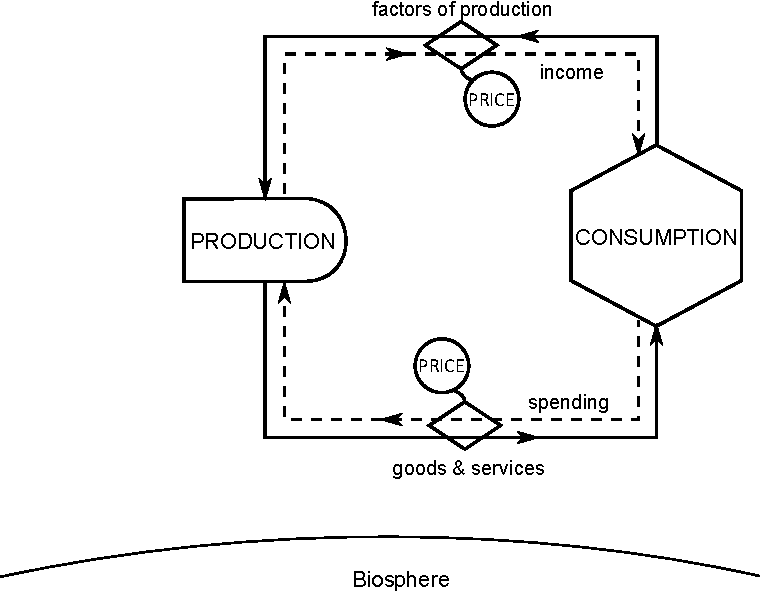
\includegraphics[width=\linewidth]{Part_0/Chapter_Introduction/images/Perpetual_motion_1.pdf}
\caption[The traditional model]{In the traditional model, the economy 
is represented as a circular flow of goods and services between two sectors. 
Producers manufacture goods and services 
by taking in labor and capital. 
Consumers exchange labor for wages 
which are used to purchase 
the goods and services of the producers.}
\label{fig:perp_motion_1}
\end{figure}

The traditional model is reflected in the economic production functions
that arose in the era of abundance. 
Economic output ($y$) was deemed to be a function 
of the factors of production (manufactured capital,~$k$, and labor,~$l$)
and augmenting technology~($A$) in the Cobb-Douglas equation:
%
\begin{equation} \label{eq:cobb-douglas}
	y = A k^{\alpha} l^\beta \; .
\end{equation}	 
%
where $\alpha$ is the output elasticity of capital, $\beta$ is the output elasticity
of labor, and $\alpha + \beta = 1$ if constant returns to scale are assumed.%
	\footnote{
	Constant Elasticity of Substitution (CES) production functions also appeared 
	in this era.
	CES productions functions have the form
	%
	\begin{equation*}
		y = A \left[ \delta_1 k \, ^\rho + (1-\delta_1) l \, ^\rho    \right]^{\frac{1}{\rho}} \; ,
	\end{equation*}
	%
	where $\delta_1$ is the factor share for capital ($k$),
	$\rho \equiv \frac{1}{1-\sigma}$, and 
	$\sigma$ is the elasticity of substitution 
	between capital ($k$) and labor ($l$).\cite{Solow:1956wj}
	Although the form of the CES model is different from 
	the Cobb-Douglas equation, 
	the functional relationship remains the same: 
	output ($y$) is a function of manufactured capital ($k$) and labor ($l$) only.
	}

In the era of abundance, 
the clockwork metaphor, 
the traditional model, 
and the Cobb-Douglas production function 
were all, in some sense, appropriate: 
capital and labor were the key drivers of economic performance.
And, national accounting reflected the binding constraints of the time. 
The first national accounting tables,
published in the United States in 1947,
were focused primarily on finanial quantifications 
of flows of capital and labor
through the economy.%
	\footnote{
	Natural resources, including energy, were, and still are, 
	included in systems of national accounts as \emph{costs}.
	They are counted in financial units
	(dollars and yen), 
	not physical units
	(barrels, tonnes, and gigajoules).
	}
**** 
MKH says: Becky, is this right? Can you provide a couple sentences
on the history here? 
And some references? 
Perhaps write about what changes have happened in the OECD SEEA.
Note that our suggested changes are already 
emerging internationally at the economy-wide scale.
There would be benefits to applying these changes at the inter-sectoral level, too.
****

Today, with the benefit of hindsight, 
we note that the clockwork metaphor and the traditional model of the economy
precluded any sort of connection 
between the economy and the biosphere.
Thus, only the internal dynamics of the economy were important.%
	\footnote{
	Because Figure~\ref{fig:perp_motion_1} has no flow of energy
	into the economy,
	we may consider the traditional model of the economy 
	to be a perpetual motion machine of the \emph{first kind}:
	the economy works without the input of energy, thus violating
	the First Law of Thermodynamics---the 
	law of conservation of energy.\cite{Rao2004}	
	}
By implication, the clockwork metaphor and traditional model 
signaled that natural resources were unimportant, 
effectively assuming that the biosphere would always provide.
If a particular natural resource became scarce, 
substitution to a different, more-readily-available resource would be made.
Wastes were quantitatively unimportant, 
effectively assuming that the biosphere had infinite assimilative capacity.
Economic forces,
through prices and the market mechanism,
were thought to effectively guide any necessary transition
within the economy.
With the clockwork metaphor, physical constraints 
imposed by the biosphere 
on allocation of resources, distribution of outputs, and 
scale of the economy 
were outside the scope of economic discussion.\cite{Daly1995}
In short, the clockwork metaphor and the traditional model of the economy 
told us that the clockwork-economy could and would carry on.

But, what happens when availability of manufactured capital and labor are no longer
the binding constraints on an economy?
The answer arrived with the era of energy constraints.


%%%%%%%%%% Era of energy constraints %%%%%%%%%%
\subsection{Era of energy constraints}
\label{sec:era_of_energy_constraints}
%%%%%%%%%%

It came as a severe shock to the economic establishment
that energy constraints brought about by the oil embargos of the early 1970s
wrought such economic havoc.
The global economy
``stalled'' due to lack of 
a single, highly-constrained resource:
fuel.
How could it be that economists were taken by surprise?

Looking back, we realize that 
all metaphors inform our thinking about the real world,
but, consequently,
they also constrain our ability to frame reality.
Erroneously, we can mistake the model-metaphor for reality, and
we interact with reality in the same manner 
as we interact with the abstract objects of our
models.%
	\footnote{
	This fallacious process is known as
	\emph{reification}; the making (\emph{facere}, Latin) real of
	something (\emph{res}, Latin) that is merely an idea.
	Alfred Whitehead refers to this as
	\emph{the fallacy of misplaced concreteness}.\cite{Whitehead2011}
	}
Classical physics told us the universe was
\emph{like} clockwork, 
so we began to interact with the universe
as if it \emph{really were} clockwork.
During the era of abundance, 
economists, guided by the clockwork metaphor,
were focused on manufactured capital and labor only;
they ignored the physical role that energy plays in the economy.

The defining characteristic of the era of energy constraints
was the scarcity, relative to demand, of fossil fuel energy resources, particularly oil.
(See Section~\ref{sec:energy-economy_coupling}.)
These energy constraints on western economies were caused
not by the depletion of oil reserves, 
but by the withholding of natural resource supply to achieve political objectives.

If they didn't already know it, economists and scientists
came to realize that input energy is required
for successful operation of the economic ``engine.''
Some saw that ignoring energy during the era of abundance
was a mistake!
The desire to include energy resources
in the economic picture
spurred the efforts of early (net) energy 
analysts.\cite{Gilliland1975, Chapman1976}
(Figure~\ref{fig:Cleveland1984} can be seen as a response
to the need to understand the role that energy 
plays in the economy.)
In the process, a machine metaphor and 
accompanying engine model for the economy 
rose to prominence.

The engine model (Figure~\ref{fig:perp_motion_2}) 
accounts for energy flows from the biosphere 
to the economy.
With the new metaphor, 
the economy changed 
from being an \emph{isolated} system~(Figure~\ref{fig:perp_motion_1}) 
to being a \emph{closed} system~(Figure~\ref{fig:perp_motion_2}). 
The importance of input energy was acknowledged, 
but wastes were still missing.
And, the biosphere was positioned as the provider of energy resources, 
the larder and gas station of the economy.\cite{Norgaard2010}

\begin{figure}[H]
\centering\
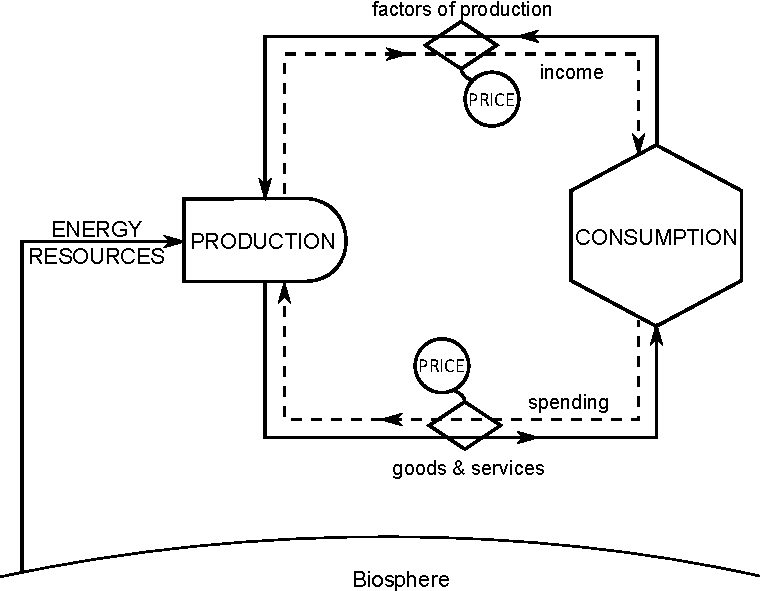
\includegraphics[width=\linewidth]{Part_0/Chapter_Introduction/images/Perpetual_motion_2.pdf}
\caption[The machine model]{The machine model of the economy includes
flows of energy into the economy from the biosphere.
This may be considered a perpetual motion machine 
of the second kind.}
\label{fig:perp_motion_2}
\end{figure}

In addition to re-evaluating the economic metaphor,
some researchers reconsidered the production function.%
	\footnote{
	It must be said that the efforts to include energy 
	as anything other than a cost of production to be evaluated in financial terms
	remain outside the economic mainstream even today.
	}
Energy augmentation of the Cobb-Douglas production function
took the form 
%
\begin{equation} \label{eq:cobb-douglas_with_energy}
	y = A k^{\alpha} l^\beta e^{\gamma}\; ,
\end{equation}	 
%
where $e$ is energy input to the economy,%
	\footnote{
	There is debate in the literature about quantification of 
	energy input to the economy ($e$).
	Most researchers use the thermal equivalent 
	of primary energy.\cite{Cleveland:1984aa, Froling:2009vo, Stern:2012ey, Nel:2010fv}
	Others use useful work obtained by efficiencies from primary exergy.\cite{Ayres:2010ug}
	}
$\gamma$ is the output elasticity of energy, and 
$\alpha + \beta + \gamma = 1$ if constant returns to scale are assumed.%
	\footnote{
	The Constant Elasticity of Substitution (CES) production function
	can be augmented with energy in several ways, 
	depending upon the desired nesting of energy relative to the other
	factors of production (capital, $k$, and labor, $l$).
	Three options exist:
	%
	\begin{equation*}
		y = \gamma \: A \: \left\{\delta \left[\delta_1 k^{-\rho_1} 
		    + (1-\delta_1)l^{-\rho_1} \right]^{\rho/\rho_1} 
		    + (1-\delta) e^{-\rho} \right\}^{-1/\rho} \; ,
	\end{equation*}
	%
	\begin{equation*}
		y = \gamma \: A \: \left\{\delta \left[\delta_1 l^{-\rho_1} 
		    + (1-\delta_1) e^{-\rho_1} \right]^{\rho/\rho_1} 
		    + (1-\delta) k^{-\rho} \right\}^{-1/\rho} \; ,
	\end{equation*}
	%
	and
	%
	\begin{equation*}
	    y = \gamma \: A \: \left\{\delta \left[\delta_1 e^{-\rho_1} 
		    + (1-\delta_1) k^{-\rho_1} \right]^{\rho/\rho_1} 
		    + (1-\delta) l^{-\rho} \right\}^{-1/\rho} \; .
	\end{equation*}
	}

In the era of energy constraints, 
the machine metaphor, 
the engine model, 
and energy-augmented production functions 
were, arguably, apt for their time:
energy was the binding constraint on the economy.
The appearance of energy in the engine model and
the energy-augmented production function
was mirrored by international efforts 
to include energy in national accounting.%
	\footnote{
	Again, we are using the term ``national accounting''
	not in the sense of systems of national accounts 
	but rather in the sense that data needs to be collected
	on the national level.
	}
The International Energy Agency (IEA) 
``\dots was founded in response to the 1973/4 oil crisis 
in order to help countries co-ordinate a collective response 
to major disruptions in oil supply.''~\cite{International-Energy-Agency:2014aa}
One of the primary objectives of the IEA is 
``to operate a permanent information system 
on the international oil market.''~\cite{International-Energy-Agency:2014aa}
Today, that ``permanent information system''~\cite{International-Energy-Agency:2014ab}
remains one of the most important 
sources of economy-level energy production and consumption
statistics in physical units.%
	\footnote{
	As opposed to financial units (currency).
	Physical units include barrels of oil, tonnes of coal, and gigajoule energy values.
	}
And, the IEA's series of World Energy Outlook 
documents~\cite{International-Energy-Agency:2014ac} is 
one of the premiere sources
of forward-looking analysis of the relationship between energy and the economy.
Although physical energy statistics and indicators
were not inserted into systems of national accounts,
the dawn of the era of energy constraints provided the impetus 
for gathering and disseminating the world's energy data.

Today, with the benefit of hindsight, 
we note that the machine metaphor and the engine model of the economy
ignored the flow of wastes from the economy to the biosphere;
the engine model still assumed that the biosphere had infinite assimilative capacity.
But, according to the Second Law of Thermodynamics, 
all real-world processes involve 
the generation of entropy
manifest as the degradation 
of material and, especially, energy resources.
High quality (low entropy) material and energy come in; 
low quality (high entropy) material and energy go out. 
Wastes exist!%
	\footnote{
	The depiction of the economy in Figure~\ref{fig:perp_motion_2} 
	can be classified as a perpetual motion machine of the second kind: 
	it perfectly converts energy resources into work (useful energy services) 
	without generating any entropy, 
	in violation of the Second Law of Thermodynamics. 	
	}
Because the generation of high entropy (low quality) output 
is a necessary feature of all processes (including economic processes), 
the generation of wastes is a normal feature of the economy, 
not an anomaly. 
The engine model had it wrong.

Furthermore, we see that the machine metaphor and the engine model of the economy
were adopted in an era where scarcity of oil supply relative to demand was caused
not by the issues associated 
with the Best First principle (Section~\ref{sec:stall_non-renewable_stocks}),
but rather 
by politically-motivated withholding of supply.
Even today, the forward-looking projections from the IEA 
(and other organizations)
continue to assume that there are effectively no physical limitations
to increasing the rate of fossil fuel extraction from the biosphere.
The presence of natural capital is acknowledged, 
but the level of the capital is not thought to constrain
the extraction rate. 
In opposition to the discussion 
in Section~\ref{sec:stall_non-renewable_stocks},
the machine metaphor and engine model assumed that 
the effects of the Best First principle 
were not a factor in economic performance.

In short, the machine metaphor and the engine model of the economy 
told us that the clockwork-economy could and would carry on,
so long as it was supplied with energy.

But, what happens when the availability of natural resources, 
especially energy,
is no longer merely a political matter?
What happens when stocks of natural resources
especially energy,
are so depleted that
it becomes too expensive for the economy to obtain them?

The answer arrived with the age of resource depletion.


%%%%%%%%%% Age of resource depletion %%%%%%%%%%
\subsection{Age of resource depletion}
\label{sec:age_of_resource_depletion}
%%%%%%%%%%

Much of Chapter~\ref{chap:intro} was spent
describing the age of resource depletion,
whose defining characteristic
is that natural capital capital constrains economic growth.
The effects of the Best First principle (exemplified by decreasing $EROI_{soc}$ for oil)
and the limited waste-assimilation capacity of the biosphere
relative to the disposal rate of materials
are now affecting the economy in ways they never did before.
England put it this way:
%
\begin{quote}
	[T]here must arrive a moment in the world's history 
	when natural capital is no longer relatively abundant and 
	human-made [manufactured] capital is no longer relatively scarce. 
	At that moment, aggregate output is no longer constrained 
	by the populations of humans [labor] and their artifacts [manufactured capital]
	and by the productivity of human effort [$A$ in 
	Equations~\ref{eq:cobb-douglas} and~\ref{eq:cobb-douglas_with_energy}]. 
	Rather, the scale of economic activity is constrained 
	by the remaining stock of natural capital and by its productivity. 
	\dots
	% Because [manufactured] capital has become relatively abundant,
	% one suspects that the economic incentive
	% to save and invest in produced capital goods would weaken.
	When this moment arrives, a new era of history has begun.\cite[p.~430]{England:2000aa}
\end{quote}
%
Prior to the age of resource depletion,
mainstream economists assumed that the ability to increase 
the rates of extraction of natural capital 
was not a factor in economic growth.
They assumed that the biosphere had infinite assimilative capacity
for the physical waste of an economy.
But, things have changed. 
Or, as we said at the end of Section~\ref{sec:consumption_unsustainable}, 
this is the end of an era.

When society transitioned from the era of abundance 
to the era of energy constraints,
three important events occurred.
(1)~The dominant economic metaphor was re-evaluated, and 
the clockwork metaphor and traditional model (Figure~\ref{fig:perp_motion_1})
were replaced by 
the machine metaphor and the engine model (Figure~\ref{fig:perp_motion_2}).
(2)~The production function was modified to include energy as a factor of production.
And, (3) national accounting changed: energy indicators and statistics 
in physical units were collected and disseminated for all countries.

All of which begs the question, 
how should the transiton 
from the era of energy constraints 
to the age of resource depletion affect 
(1)~society's dominant metaphors for and models of the economy,
(2)~the production function, and 
(3)~national accounting?
In the next section, we argue for a new metaphor, 
and the heart of this book (Chapters~\ref{chap:materials}--\ref{chap:intensity})
provides a theoretical grounding for national accounting in the age of resource depletion.
The way forward on production functions
is beyond the scope of this text.%
	\footnote{
	But, see England for a starting point.\cite{England:2000aa}
	}


%%%%%%%%%% Economy is society's metabolism %%%%%%%%%%
\section{The economy is society's metabolism}
\label{sec:economy_metabolism}
%%%%%%%%%%

In our opinion, an apt metaphor for the economy should provide for robust interaction
and suggest tight coupling between the biosphere and the economy. 
Specifically, it should account for the following facts about real economies. 
Economies:

\begin{enumerate}
	\item{\label{itm:intake}intake material and energy from the biosphere}
	\item{\label{itm:internal_exchange}exchange materials, energy, and information internally}
	\item{\label{itm:discharge}discharge material and energy wastes to the biosphere}
	\item{\label{itm:energetic_costs}are affected by energetic costs}
	\item{\label{itm:scarcity}are affected non-linearly by scarcity 
			in the face of low substitutibility}
	\item{\label{itm:non-linear}can change non-linearly or in discrete steps with the potential 
			for structural transformation}
	\item{\label{itm:embodies}accumulate embodied energy in material stocks, and}
	\item{\label{itm:robust}maintain organizational structure despite changes 
			in their environment.%
				\footnote{We note that 
				several areas of the literature speak to the items in this list.
				Materials Flow Analysis~(MFA) and 
				Economy-Wide Materials Flow Analys~(EW-MFA)
				stress the importance of
				material intake by the economy. 
				(See Section~\ref{sec:materials_auto}.)
				The Input-Output~(I-O) method highlights the effects of internal exchanges
				of material and information with economies. 
				(See Chapter~\ref{chap:intensity}.)
				Life-Cycle Assessment~(LCA) techniques focus attention 
				on otherwise-neglected wastes. 
				(See Section~\ref{sec:intensity_auto}.)
				Net Energy Analysis~(NEA) predicts that energy resource 
				scarcity reduces Energy Return on Investment~(EROI)
				and increases energy prices.
				(See Sections~\ref{sec:B_energy} 
				and~\ref{sec:resource_quality_and_irreversibility}.)
				The Energy Input-Output~(EI-O) method gives prominence to energetic costs
				of internal material and energy flows.
				(See Chapter~\ref{chap:intensity}.)
				And, thermodynamic control-volume modeling describes
				transient behavior and system transformations.
				(See Chapters~\ref{chap:materials}--\ref{chap:value}.)
			}}
\end{enumerate}

Metabolisms%
	\footnote{The 
	Greek root of metabolism 
	(\emph{metabol$\bar{e}$}) means ``change.''}
exhibit the characteristics in the list above.
Metabolisms and the organisms they support
are intimately connected with the biosphere:
they withdraw materials and energy from the biosphere~(\ref{itm:intake}), 
transfer materials and energy internally via metabolic processes~(\ref{itm:internal_exchange}),
and discharge wastes back to the biosphere~(\ref{itm:discharge});
in fact, their very survival depends on these processes.
Extending Figures~\ref{fig:perp_motion_1} and~\ref{fig:perp_motion_2}
to include the facts in items~(\ref{itm:intake})--(\ref{itm:discharge}), % chktex 36
we obtain Figure~\ref{fig:metabolic_economy}.
Metabolisms are affected by energetic costs~(\ref{itm:energetic_costs}): 
an organism that obtains less energy than it expends is doomed.
Withholding life-sustaining resources brings drastic, non-linear
consequences for any metabolism~(\ref{itm:scarcity}).
Metabolisms enable non-linear, structural transformations
in their host organisms (e.g., metamorphosis, puberty, and evolution)~(\ref{itm:non-linear}).
And, energy absorbed by a metabolism is considered to be ``embodied''
in the cells of the organism~(\ref{itm:embodies}).
Metabolisms exist in a state of dynamic stability~(\ref{itm:robust}),
adjusting and readjusting to maintain their internal conditions
despite changes in the environment;
for a metabolism, equilibrium means death!

The economy is society's metabolism.

\begin{figure}[!ht]
\centering\
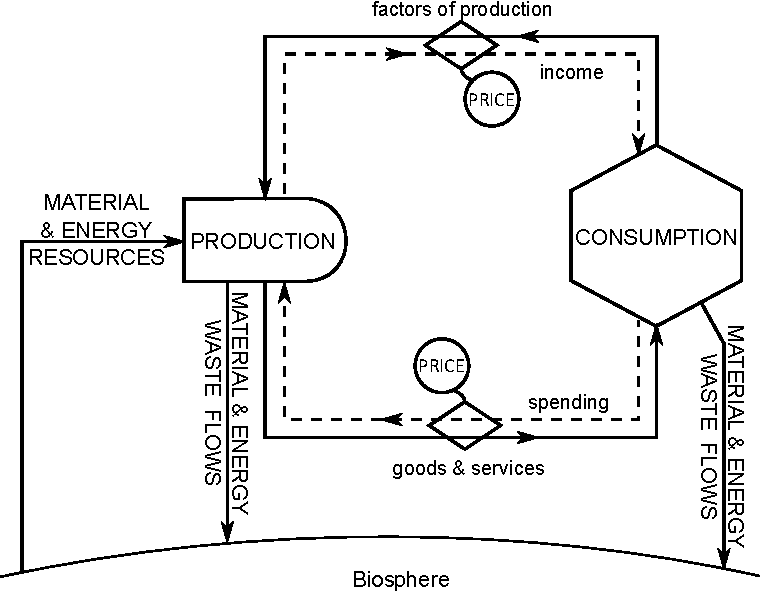
\includegraphics[width=\linewidth]{Part_0/Chapter_Introduction/images/PERKS.pdf}
\caption[The metabolism model]{The metabolism model provides a comprehensive view 
of the economy, fully consistent with the laws of thermodynamics, 
including degraded resources (waste) expelled 
to the environment as a necessary consequence of economic activity.}
\label{fig:metabolic_economy}
\end{figure}

Although we're not the first to suggest the metabolism metaphor for the economy
\cite{Liu2012, Giampietro2000, Giampietro2013, F-K1999, F-K2003, Heijman:1988aa},
**** Mik--add Gowdy references? ****
we believe that
the metabolism metaphor is under-utilized 
on both practical and theoretical levels.
On the practical level, the metabolism metaphor is under-utilized
because national accounting, to date, 
is built upon the machine metaphor and engine model for the economy
(Section~\ref{sec:era_of_energy_constraints}).
This book attempts to correct that oversight 
by using the metabolism metaphor 
to develop a rigorous theoretical framework 
for comprehensive national accounting.
(See Chapters~\ref{chap:materials}--\ref{chap:intensity}.)
On a theoretical level, the metabolism metaphor is under-utilized because 
most researchers (with the exception of Giampietro~\cite{Giampietro2000, Giampietro2013})
use the metabolism metaphor merely as as framing device for analyses of
raw material flows into the economy for the purpose of understanding 
stocks of raw materials in the biosphere.%
	\footnote{The field most closely associated with the metabolism metaphor is
	Materials Flow Analysis (MFA). 
	To be fair, materials flow analysts clearly acknowledge that 
	materials flow into the economy (minerals and ores, especially),
	in part,
	for the purpose of building up stocks of technical infrastructure (buildings),
	livestock, and people.\cite[p.~116]{F-K1999} 
	However, there is little emphasis on quantifying \emph{levels} 
	of material stock in Materials \emph{Flow} Analysis, 
	as its name implies.
	In fact, the equations in MFA~\cite[Equation~1]{F-K1999} are almost always written as%
	\begin{equation*}
		\mathrm{inflow} = \mathrm{outflow} + \mathrm{accumulation \; ,}
	\end{equation*}
	reflecting the focus on material inflow to the economy.
	In this book, similar equations 
	(see Equation~\ref{eq:general_accumulation_equation}) 
	are written as%
	\begin{equation*}
		\mathrm{accumulation} = \mathrm{inflow} - \mathrm{outflow \; ,}
	\end{equation*}
	thereby focusing on accumulation of stocks within the economy.
	}
Those who employ the metabolism metaphor
tend to focus little attention on capital stock within the economy itself.
In effect, this is the same oversight as national accounting: 
under-appreciation of the important role of capital
in determining material and energy demand 
for the emplacement, use, maintenance, and replacement of the very same capital.

It becomes a vicious cycle. 
By not accounting for capital stock on a physical basis 
in national accounting, 
society is unable to appreciate 
the important physical role that capital stock plays in the economy
(Section~\ref{sec:stall_capital_stock}).
Because society under-appreciates the physical role of capital stock in the economy, 
there is little urgency to begin accounting 
for manufactured capital on a physical (rather than financial) basis.

We think that a deeper understanding of the metabolic metaphor
can serve to both highlight the important physical role of manufactured capital stock and 
provide the basis for a rigorous theoretical framework 
for comprehensive national accounting.
In the following sections, 
we deepen the metabolism metaphor by considering 
anabolism (capital formation),
catabolism (energy production),
autophagy (recycling), and
issues of scale.
Thereafter, we summarize the benefits of the metabolism metaphor
for national accounting.

%+++++++++ Anabolism ++++++++++
\subsection{Anabolism (capital formation)}
\label{sec:anabolism}
%+++++++++

Metabolic processes are classified as anabolic and catabolic 
(Section~\ref{sec:catabolism}).
Anabolic processes build up materials within the body (bones, muscles, tissues).
For example, anabolic steroids are hormones that stimulate 
the human body's natural muscle and bone growth processes.
Anabolic processes are fueled by the breakdown 
of adenosine triphosphate (ATP), the cellular energy source.
Raw materials for anabolic processes are provided by food, 
which, ultimately, comes from the biosphere.

The economic analog to biological anabolism is capital formation, 
net addition to the stock of capital within a period of time.
Traditionally, capital formation is measured in currency units.
Thus, capital formation is the financial evidence 
of the emplacement of manufactured infrastructure.
Whereas biological anabolism is fueled by ATP, 
capital formation is fueled by the energy sector of the economy.
The raw material for capital formation comes to the 
economy from the biosphere.

We discuss extraction and use of materials in Chapter~\ref{chap:materials}
and the importance of capital stock throughout the book.


%+++++++++ Catabolism ++++++++++
\subsection{Catabolism (energy production)}
\label{sec:catabolism}
%+++++++++

Catabolic processes break down and destroy material stocks within an organism
through an oxidation process.
At the cellular level, catabolic oxidation releases chemical free energy, 
some of which synthesizes adenosine triphosphate (ATP), 
thereby providing fuel to cells. 
The rest of the released energy is manifest as waste heat.
One of the waste products of cellular catabolism is CO$_2$.

The analogy between catabolic processes and the work 
of the energy sector in the economy is striking.
Power plants (fired by coal, oil, and natural gas) break down fossil fuels
in an oxidation process (combustion) to produce useful energy 
(typically, electricity or mechanical drive~\cite{Ayres:2010ug}), 
thereby providing energy to other sectors of the economy.
Both waste heat and CO$_2$ are byproducts of combustion, 
and O$_2$ is consumed in the process.

We focus on energy production in the economic context 
in Chapter~\ref{chap:direct_energy}.


%+++++++++ Autophagy ++++++++++
\subsection{Autophagy (recycling)}
\label{sec:autophagy}
%+++++++++

One catabolic pathway, autophagy, 
involves the breakdown of damaged, unneeded, or dysfunctional cellular components 
(proteins and cell organelles)
for the purpose of re-use within the organism. 
Autophagy can be an adaptive response to low calorie intake,
promoting cell survival.

Again, the analogy between cellular metabolism and the economy is striking.
Whereas cellular autophagy repurposes proteins and cell organelles
for re-use by an organism,
recycling repurposes degraded
yet economically-valuable materials
for re-use by the economy.
Furthermore, recycling can also be an adaptive response 
to reduced material and energy inputs.
One famous example can be found on the streets of Cuba.
In the face of economic sanctions,
government restrictions on vehicle purchases, and
high import tariffs,
automobile imports by Cuba are very low.
As a result, Cuba hyper-recycles autos that were imported
prior to sanctions and manufactures replacement parts locally.
The average lifespan of automobiles has been extended
such that an estimated 60,000, pre-1960 cars~\cite{Schweid:2004aa} 
(so-called ``yank tanks'') are in service on the island.%
	\footnote{Despite the recent change allowing new car purchases by individuals,
	astronomical import taxes mean that Cuban streets remain populated 
	with vintage 1950s autos.\cite{Ramey:2014aa}
	}
(See Figure~\ref{fig:vintage_autos_cuba}.)

\begin{figure}[!ht]
\centering\
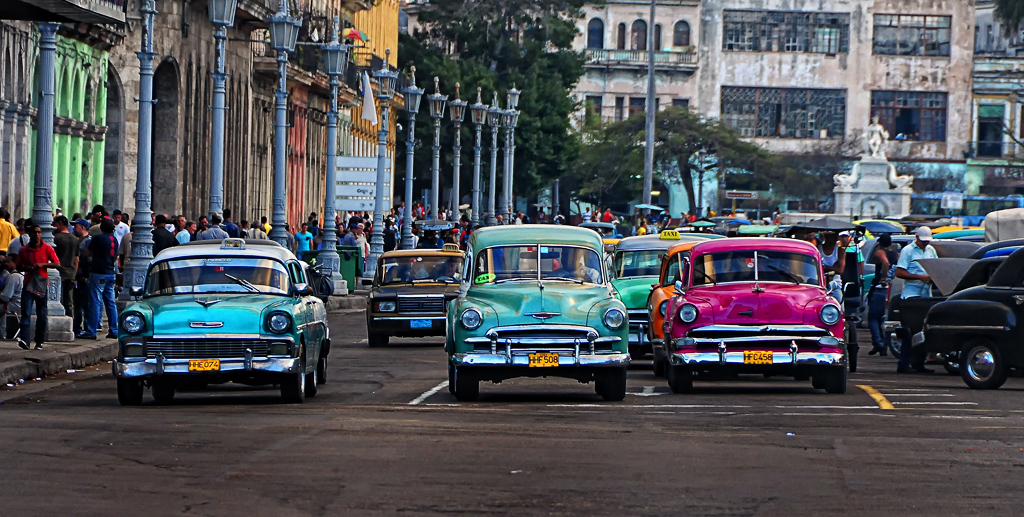
\includegraphics[width=\linewidth]{Part_0/Chapter_Acct_For_WoN/images/old-cars-of-cuba-dsc_4474-1024.jpg}
\caption[Vintage autos in Cuba]{Vintage autos (``yank tanks'') in Cuba (2011).

**** 

This image is from 

\url{http://lcowlesphotography.wordpress.com/2011/02/13/old-cars-of-cuba/}.

What must we do to obtain the rights to the image? 
If we can't obtain rights to Figure~\ref{fig:vintage_autos_cuba}, 
other options include:

\url{http://myadventuresacrosstheworld.wordpress.com/2013/03/14/transportation-in-cuba-old-cars-historical-cars-cocotaxi-bicitaxi-camionetas-and-what-not/}

\url{http://www.travelforboomers.com/2012/10/17/so-close-and-yet-so-far-away-viva-cuba/}

\url{http://ocean.otr.usm.edu/~w301497/travels/cuba2010/cuba2010b.html}

****}
\label{fig:vintage_autos_cuba}
\end{figure}

It's not difficult to imagine that dynamics similar to Cuba's will emerge
if the inflow rate 
of any important natural but recyclable resource 
is reduced to a trickle
by the effects of depletion.%
	\footnote{
	See Section~\ref{sec:stall_non-renewable_stocks}
	for a discussion of depletion of a non-recyclable natural resource, oil.	
	}

Regardless of the origin of material constraints, 
the effect on the economy will be the same:
re-use, recycling, and, where possible, substitution to other resources
will become increasingly imperative.

We focus on recycling in Section~\ref{sec:recycling}.


%+++++++++ Scale ++++++++++
\subsection{Issues of scale}
\label{sec:metabolic_scale}
%+++++++++

The metabolism metaphor brings to light issues of scale (size)
for economies and societies.
First, scale is directly related to material flow rates.
Larger organisms consume food at higher rates,
in part to obtain essential nutrients to replenish cellular structures.
Similarly, economies with higher levels of emplaced capital
require larger material flow rates to provide 
raw materials to machines and food to people.
(See Section~\ref{sec:stall_capital_stock} for more on this topic.)

In Figure~\ref{fig:Kleiber_law},
we see Max Kleiber's empirically-determined relationship between
metabolic rate (heat production, in kcal/day) and
animal mass (in kg)
plotted on a log-log scale
for a variety of animals,
from mice to whales.
Green dots show data points, and
lines represent theoretical scaling due to either mass (weight)
or surface area.
The best fit to the data (red line)
passes between the weight and surface area lines.

\begin{figure}[!ht]
\centering\
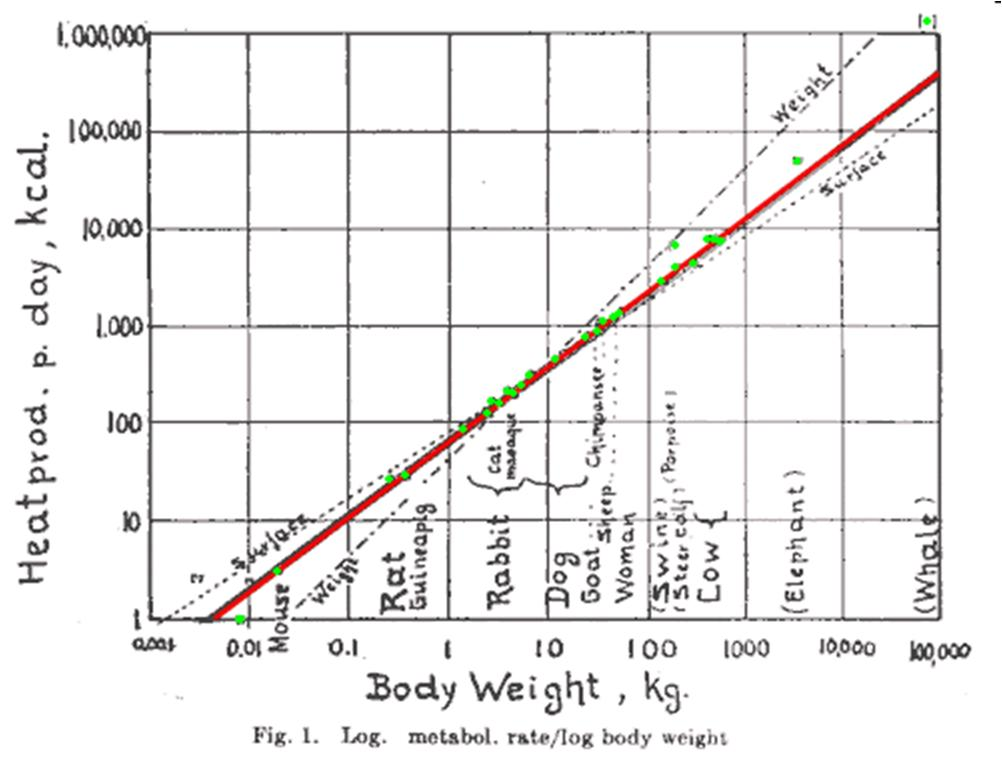
\includegraphics[width=\linewidth]{Part_0/Chapter_Acct_For_WoN/images/Kleiber1947.jpg}
\caption[Kleiber's law for metabolic rates of animals]{Kleiber's law 
for metabolic rates (heat production) of different-sized animals~\cite[p.530]{Kleiber1947}.
Larger animals, as determined by mass, have a higher metabolic rate, 
but the relationship between mass and metabolic rate is not linear.

**** Do we need to obtain permission to use this figure? ****}
\label{fig:Kleiber_law}
\end{figure}

Kleiber's law which states this relationship mathematically,
is defined as
%
\begin{equation}\label{eq:Kleiber_law}
	\dot{Q} = q_{0} m^{3/4}
\end{equation}
%
where 
$\dot{Q}$ is metabolic rate (heat production),
$m$ is the mass of the animal, and
$q_{0}$ is a mass-independent normalization constant.
From Equation~\ref{eq:Kleiber_law},
we see that doubling the mass increases the metabolic rate by
$2^{3/4} = 1.68$ times.
To compensate for higher rates of heat loss due to high surface area-to-volume ratio,
small animals have proportionally higher metabolic rates
and proportionally larger food requirements.

If the economy is society's metabolism and 
the scale of an organism corresponds to the inventory 
of capital stock in an economy, 
the metabolism metaphor suggests that larger economies 
will require a higher rate of energy supply.
In fact, we know this to be true.
Built-out, industrialized economies with higher levels of emplaced capital
(those with more roads, cars, and buildings)
tend to consume energy at a higher rate, 
both in an absolute sense and on a per-capita basis,
compared to developing economies.


%%%%%%%%%% Metabolism metaphor helps %%%%%%%%%%
\subsection{Benefits of the metabolism metaphor}
\label{sec:metabolism_helps}
%%%%%%%%%%

The metabolism metaphor is compelling, 
because it helps us to see more clearly
and understand more deeply
how the real economy operates.
But how does the metabolism metaphor lead us to a better understanding 
of the coupling between the biosphere and the economy 
and provide guidance for more-comprehensive national accounting?
We think so.

In terms of a better understanding of the economy, 
the metabolism metaphor teaches us that the economy is a biophysical entity
that requires both materials and energy for survival.
We learn that economic activity is \emph{natural}.
It can be likened to breathing (respiration): 
O$_2$ is consumed as CO$_2$ is produced.
It can be likened to digestion:
raw materials and chemical potential energy are ingested, 
the body grows, 
and energy is provided for everyday activities.
Just as food from the biosphere provides materials and energy for
anabolic and catabolic processes in an organism, 
materials and fuels from the biosphere provide matter and energy for
capital formation and energy production in society.
Without materials and energy from the biosphere, 
metabolisms fail and organisms die. 
Without materials and energy from the biosphere,
the economies collapse and societies fade away.
In short, the economy is coupled to the biosphere,
because it is utterly and completely dependent upon it.

The metabolism metaphor teaches us that 
larger economies demand increasingly higher
material and energy flow rates from the biosphere.
We see that limits to economic growth
are both possible and expected.
From the metaphor we learn that economic ``stall'' is not pathological, 
but natural, especially in mature economies 
that have encountered some type of biophysical limit.
(See Section~\ref{sec:stall_non-renewable_stocks}.)
We might expect to encounter any number of limits:
supply rates of materials from the biosphere,
supply rates of energy from the biosphere,
scale of the economy relative to the biosphere.
In the metabolism metaphor, autophagy indicates that stocks 
of capital within society are reservoirs of 
material and (embodied) energy that can and should be 
broken down and re-used or re-purposed,
rather than discarded, 
when out of service.

Through an understanding of the deep interconnectedness and complexity
of organisms and species in the biosphere, 
we come to appreciate the interdependence 
among actors within and sectors of the economy.
Furthermore, an appreciation of the complex nature of economies leads us 
to acknowledge the difficulty in discerning
precisely which limit(s) is (are) encountered when growth stalls.
In fact, there is no single explanation 
for the slowdown of growth in OECD economies 
discussed in Section~\ref{sec:growth_has_slowed}.
The best explanation to date involves many intertwining factors: 
slowing growth of energy input rate, 
decreasing energy return on investment in the liquid fuel sector,
problems in the credit markets, etc.

In terms of national accounting, 
a deeper understanding of the metabolism metaphor 
will lead to significant changes in national accounting.
It will lead us to acknowledge
the important role of \emph{both} flows 
(e.g., GDP, 
rates of material and energy extraction from the bioshere,
rates at which money spins through the economy)
\emph{and} stocks 
(e.g., manufactured capital, monetary savings, non-renewable energy supplies).
Furthermore, appreciation of the physical basis of the real economy will lead us 
to account for both stocks and flows 
in physical units (kg and kJ) as well as financial units (currency).

Deeper understanding of the metabolic metaphor will
lead systems of national accounts to become
focused as much on stocks as on flows.
Systems of national accounts will expand beyond financial accounting
to become a compendia of both physical as well as financial assets
of an economy.
By counting flows \emph{and} stocks 
in both physical and monetary units,
national accounting will provide a comprehensive picture 
of the \emph{health} and \emph{wealth} of economies, respectively.


%%%%%%%%%% Rigorous framework %%%%%%%%%%
\section{New national accounting}
\label{sec:new_national_accounting}
%%%%%%%%%%

Society needs to respond 
to the material and energy shortages that
we now face (Chapter~\ref{chap:intro}),
and part of that response
should involve more-comprehensive national accounting 
guided by a deeper understanding of the real economy 
gained through the metabolism metaphor (Section~\ref{sec:economy_metabolism}).
It is imperative that we begin now
to help society deal with impending biophysical limits.

But how? 
What should we be counting and in what units?
And, how should the data be analyzed?

Firm theoretical grounding is needed 
\emph{before} we begin the process of expanding national accounts.
We need a framework, a way to organize our thoughts about the notion 
of national accounting in the age of resource depletion.
This book is an attempt to provide just that: 
a theoretical framework
for comprehensive national accounting
in the age of resource depletion
that could be adopted in systems of national accounts.

The first question above (``What should we be counting and in what units?'') 
is the topic for the remainder of this section,
and the answer provides the structure for the heart of the book.
The second question above (``How should the data be analyzed?'')
is the topic of Chapter~\ref{chap:intensity}.

We believe the key to understanding society's metabolism
in the age of resource depletion is to understand how 
materials, energy, embodied energy, and economic value
each interacts with the economy.
Specifically, it is important to understand how each
accumulates within the economy and how each flows into, within, and out of the economy.
The first three items (materials, energy, and embodied energy) are
inspired directly by the metabolism metaphor.
The fourth item (economic value) is necessary to understand the way 
that the lifeblood of economies (currency) flows through the economy.
Of course, each of the items in the list interacts with the others 
and the biosphere dynamically.
If we can begin to carefully track these items, 
we will be on our way toward gathering the information necessary to 
expand national accounting.

Systems of national accounts that are informed by the metabolism metaphor 
and account for materials, energy, embodied energy, and economic value
may allow consumers, producers,
and policy-makers to answer critical questions that are not
answerable today, such as:

**** Do we like the questions bold? ****

\begin{enumerate}
	\item{\textbf{How much energy was used in the manufacture and transport
				of two competing goods in the supermarket?} 
				(Or, equivalently, how much energy is embodied 
				in two competing goods in the supermarket?)}
	\item{\textbf{What might be the optimal scale of an economy in terms of GDP 
				and what are the impacts of an optimally-sized economy on natural capital?}}
    \item{\textbf{How is scarce fossil fuel dependency embedded 
    			in the interlocking fabric of the economy?}} 
    \item{\textbf{How will economies that are dependent on coal, oil, 
     			and other forms of non-renewable energy transition 
    			to renewable forms of energy?}}
	\item{\textbf{How might an economy be affected as an increasing share of production
				is directed toward replacing 
				degraded ecosystem services?}~\cite[p.~221]{kummel2011}​}
\end{enumerate}

Our approach to developing a rigorous theoretical foundation for 
comprehensive national accounting is to
develop a dynamic model 
by applying rigorous thermodynamics 
to materials and energy flows into, among, 
and out of economic sectors,
informed by the metabolism metaphor,
in a manner that is verifiable against 
the existing (or expanded) 
national accounts.


%%%%%%%%%% Structure %%%%%%%%%%
\section{Structure of the book}
\label{sec:structure}
%%%%%%%%%%

The list of items to be accounted 
(materials, energy, embodied energy, and economic value)
provides structure for our proposed framework
and much of the rest of this book.

Part~\ref{part:matter} addresses flows of physical matter and energy
through the economy.
Chapter~\ref{chap:materials} discusses material flows and accumulation.
Flows of energy are covered in Chapter~\ref{chap:direct_energy}, 
and a rigorous, thermodynamics-based definition of and accounting for 
embodied energy is presented in Chapter~\ref{chap:embodied_energy}.

In Part~\ref{part:values}, we turn to flow and accumulation of 
non-physical entities through the economy. 
Flows and accumulation of economic value are discussed in Chapter~\ref{chap:value}.
In Chapter~\ref{chap:intensity}, we combine the results from 
Chapters~\ref{chap:embodied_energy} and~\ref{chap:value} to
develop an important indicator of economic activity:
the energy intensity of economic production.

Part~\ref{part:implications} gives context to the framework developed in
Parts~\ref{part:matter}~and~\ref{part:values}.
Chapter~\ref{chap:implications} draws out some of the direct implications
of our model.
Chapter~\ref{chap:unfinished_business} looks at 
unfinished business: practical, conceptual, and theoretical issues
that arise in the development of our new model.
And, we end with a summary in Chapter~\ref{chap:summary}.

Throughout the methodological chapters~(\ref{chap:materials}--\ref{chap:intensity}),
our accounting framework is developed
through a series of increasingly-disaggregated
models of the economy~(Table~\ref{tab:examplesABC}),
and we use the US auto industry 
as a running example for application and discussion.

\begin{table}
\caption[Examples used throughout this book]{Examples
used throughout this book.}
\begin{center}
  \begin{tabular}{c @{\hspace{1.5em}} c @{\hspace{1.5em}} c @{\hspace{1.5em}} c @{\hspace{1.5em}} c}
    \toprule
    Example & Sector 0 & Sector 1 & Sector 2 & Sector 3 \\ 
	\midrule
    A & Biosphere	&	Society            & NA         & NA                 \\
    B & Biosphere	&	Final Consumption  & Production & NA                 \\
    C & Biosphere	&	Final Consumption  & Energy     & Goods \& Services  \\
  \bottomrule
  \end{tabular}
\end{center}
\label{tab:examplesABC}
\end{table}
 
**** 

The next two paragraphs are duplicated from 
Section 3.5 (Materials in the US Auto Industry).
We duplicated them here temporarily so that the editors can 
see the purpose of and justification for the auto industry example. 

****

The running example of the US auto industry demonstrates that our dynamic model 
can be tied into national accounts.
The US auto industry example shows where data are available 
(e.g., economic value, Chapter~\ref{chap:value}), 
where it is old (e.g., energy intensity, Chapter~\ref{chap:intensity}), 
and where it has never been available 
(e.g., accumulated embodied energy, Chapter~\ref{chap:embodied_energy}).  
The US auto industry is, therefore, 
illustrative of the challenges inherent 
in obtaining data that would feed the model.

The auto industry 
has been used previously
in the literature in both 
process-based~\cite{Berry:1973vo, Sullivan1995, Stodolsky1995, 
							Sullivan1998, McCleese2002, Sullivan2010, Hawkins2012}
and Input-Output~\cite{Bullard:1978vd, MacLean1998, MacLean2003}
analysis methods,
Furthermore, the industry
remains a large portion of many industrialized economies, 
is very resource intensive, 
has obvious links with energy because
its health is sensitive to disruptions in energy supplies, and
the industry also shows evidence of 
post-industrial decline (shrinking profit margins, etc.).



\bibliographystyle{unsrt}
\bibliography{../../Metabolic}






%%%%%%%%%%%%%%%%%%%%%%%%%%%%%%%%%%%%%%%%
%%%%%%%%%%%%%%%%%%%%%%%%%%%%%%%%%%%%%%%%
% BONEPILE
%%%%%%%%%%%%%%%%%%%%%%%%%%%%%%%%%%%%%%%%
%%%%%%%%%%%%%%%%%%%%%%%%%%%%%%%%%%%%%%%%

% %%%%%%%%%% Metaphors and Models %%%%%%%%%%
% \section{Metaphors and models}
% \label{sec:metaphors_and_models}
% %%%%%%%%%%
%
% As discussed in Section~\ref{sec:new_accounting},
% national accounting is incomplete, and
% an objective for this book is to provide rigorous theoretical grounding for
% a better national accounting framework.
%
% **** The motivation for this comes from looking at the history
% of how society has determined what should be incuded in national accounts.
% Change the
%
% The need for this is obvious when we look the vision society has for national accounts.
% ****
%
% But, before moving ahead with developing that framework,
% it is useful to consider how society has come to this point.
% How is it that we don't routinely and comprehensively account for
% important material and energy flows into, within, and out of the economy
% on a physical basis in systems of national accounts?
%
% The classical economists certainly appreciated the dependence of
% economic activity on biophysical processes.\cite{Hall2011, Cleveland1987, Dale2012}
% However, somewhere between William Stanley Jevons' 1865
% assessment that
% ``the very existence of Britain, as a great nation''~\cite[IV.3]{Jevons1865}
% was tied to a continued supply of low-cost coal
% and Julian Simon's 1998 statement that
% ``natural resources are not finite in any economic sense,''~\cite[p.~54]{Simon1998} %chktex 38
% the importance of the biosphere was lost.
% In the following sections, we argue that
% a contributing reason for incomplete national accounting
% is that we have the wrong metaphor for the economy,
% and we provide a suggestion for improvement.
%
%
% %+++++++++ The clockwork metaphor ++++++++++
% \subsection{The clockwork metaphor}
% \label{sec:clockwork_metaphor}
% %+++++++++
%
% Most economics textbooks today depict the economy
% as in Figure~\ref{fig:perp_motion_1}.
% Goods and services flow from the production sector
% to the household sector~(consumption)
% in exchange for payments.
% The factors of production (labor and capital)
% flow from the household sector to the
% production sector in exchange for wages and rents (income).
% Attention is primarily focused on the circular flow
% of money~(dashed line).
%
% \begin{figure}[!ht]
% \centering\
% 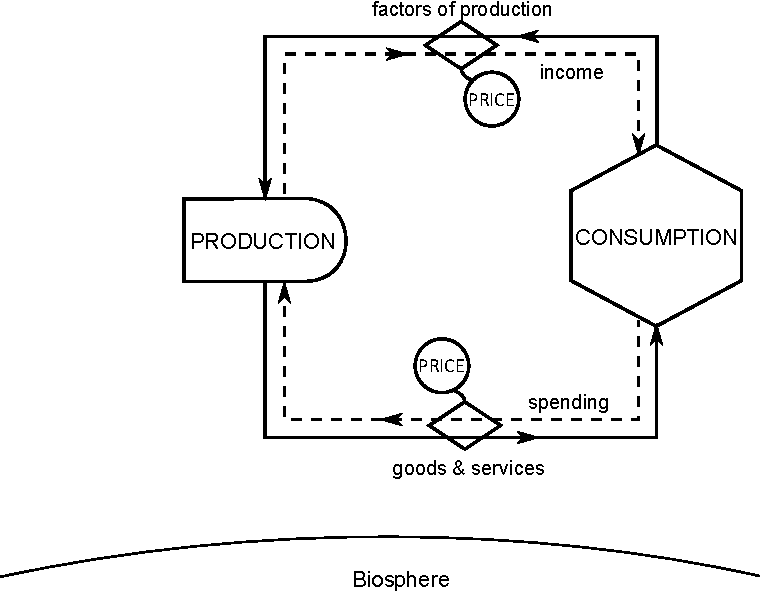
\includegraphics[width=\linewidth]{Part_0/Chapter_Introduction/images/Perpetual_motion_1.pdf}
% \caption[The traditional model]{In the traditional model, the economy
% is represented as a circular flow of goods and services between two sectors.
% Producers manufacture goods and services
% by taking in labor and capital.
% Consumers exchange labor for wages
% which are used to purchase
% the goods and services of the producers.}
% \label{fig:perp_motion_1}
% \end{figure}
%
% This traditional model of the economy~(Figure~\ref{fig:perp_motion_1})
% is unashamedly mechanistic.
% General equilibrium models of the economy
% ~\cite{Walras1892, Walras1993}
% were borrowed directly from classical physics' models of
% mechanical equilibrium which, in turn, arose from the
% ``clockwork universe'' metaphor.\cite{Ingrao1990}
% The clockwork metaphor is a simplification
% that helps us make sense of the world around us.
% Like all metaphors, it informs our thinking about the real world,
% but, consequently,
% it also constrains our ability to frame reality.
% Erroneously, we mistake the model-metaphor for reality, and
% we interact with reality in the same manner
% as we interact with the abstract objects of our
% models.\footnote{This fallacious process is known as
% 	\emph{reification}; the making (\emph{facere}, Latin) real of
% 	something (\emph{res}, Latin) that is merely an idea.
% 	Alfred Whitehead refers to this as
% 	\emph{the fallacy of misplaced concreteness}.\cite{Whitehead2011}
% 	}
% Classical physics told us the universe was
% \emph{like} clockwork,
% so we began to interact with the universe
% as if it \emph{really were} clockwork.
% It then became easy to collect economic data that confirmed the clockwork model,
% because the model told us which data to collect.
%
% The clockwork metaphor and the traditional model of the economy
% preclude any sort of connection
% between the economy and the biosphere.
% Thus, only the internal dynamics of the economy are important.
% They tell us that natural resources are unimportant,
% effectively assuming that the biosphere will always provide.
% If a particular resource becomes scarce,
% substitution to a different, more-readily-available resource will be made.
% Wastes are quantitatively unimportant,
% effectively assuming that the biosphere has infinite assimilative capacity.
% Economic forces (through prices and the market mechanism)
% are thought to effectively guide any necessary transition
% within the economy.
% With the clockwork metaphor, physical constraints
% imposed by the biosphere
% on allocation of resources, distribution of outputs, and
% scale of an economy
% are outside the scope of neoclassical economic discussion.\cite{Daly1995}
% In short, the clockwork metaphor and the traditional model of the economy
% tell us that the clockwork-economy can and will carry on.
%
% In light of the discussion in Chapter~\ref{chap:intro},
% the clockwork metaphor and traditional model of the economy
% are clearly problematic.
% Because Figure~\ref{fig:perp_motion_1} has no flow of energy
% into the economy,
% we may consider the traditional model of the economy
% to be a perpetual motion machine of the \emph{first kind}:
% the economy works without the input of energy, thus violating
% the First Law of Thermodynamics---the
% law of conservation of energy.\cite{Rao2004}
%
%
% %%%%%%%%%% Machine metaphor %%%%%%%%%%
% \subsection{The machine metaphor}
% \label{sec:machine_metaphor}
% %%%%%%%%%%
%
% The limits of the clockwork metaphor and traditional model of the economy were
% exposed by the oil shocks of the 1970s.
% The global economy
% ``stalled'' due to lack of
% a single, highly-constrained resource:
% fuel.
% Many came to realize that input energy is required
% for successful operation of an economic ``engine.''
% Thus, a machine metaphor and
% accompanying engine model for the economy
% rose to prominence
% in the late 1970s and early 1980s.
% The need to include energy resources
% in the economic picture
% spurred the efforts of early (net) energy
% analysts.\cite{Gilliland1975, Chapman1976}
%
% The engine model (Figure~\ref{fig:perp_motion_2})
% accounts for energy flows from the biosphere
% to the economy.
% With the new metaphor, the economy changed from
% an \emph{isolated} system~(Figure~\ref{fig:perp_motion_1}) to
% a \emph{closed} system~(Figure~\ref{fig:perp_motion_2}).
% The importance of input energy was acknowledged,
% but wastes are missing.
% And, the biosphere is relegated to the position
% of provider of energy resources;
% the larder and gas station of the economy.\cite{Norgaard2010}
%
% \begin{figure}[H]
% \centering\
% 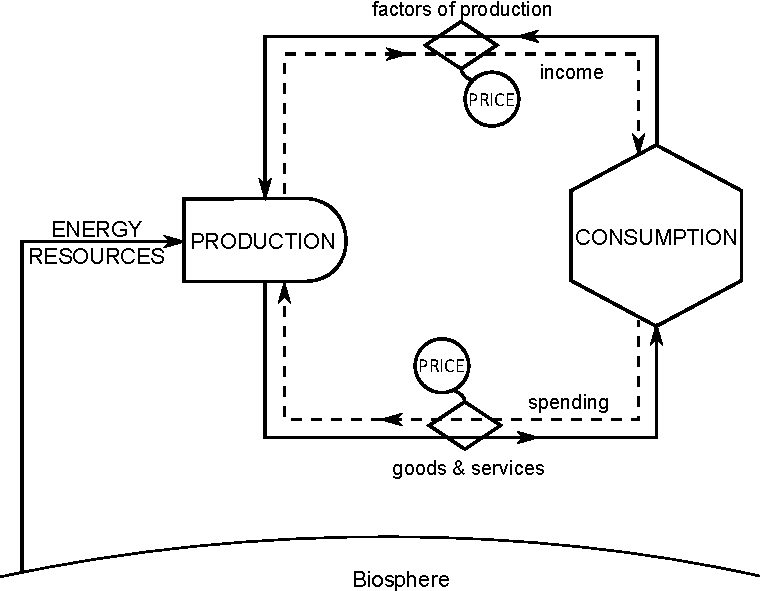
\includegraphics[width=\linewidth]{Part_0/Chapter_Introduction/images/Perpetual_motion_2.pdf}
% \caption[The machine model]{The machine model of the economy includes
% flows of energy into the economy from the biosphere.
% This may be considered a perpetual motion machine
% of the second kind.}
% \label{fig:perp_motion_2}
% \end{figure}
%
% The machine metaphor and engine model,
% like the clockwork metaphor and traditional model,
% are mechanistic.
% Much like the engines of the Industrial Revolution,
% the economic engine is assumed to be well-behaved and amenable to control.
% Even today, machine metaphors abound in our economic discussions.
% We continue to speak of ``fueling'' the ``economic engine''
% lest it should ``stall.''~\cite{Liu2012}
% Like a well-running engine, the economy is assumed
% to be resilient to small or even quite large perturbations.
% It can either self-correct,
% or be corrected predictably with adjustments to
% a few policy levers.
%
% But how accurate is the engine model?
%
% According to the Second Law of Thermodynamics,
% all real-world processes involve the degradation
% of material and, especially, energy resources
% and the creation of entropy.
% High quality (low entropy) material and energy come in;
% low quality (high entropy) material and energy go out.
% Wastes exist!
% The depiction of the economy in Figure~\ref{fig:perp_motion_2}
% can be classified as a perpetual motion machine
% of the \emph{second kind}:
% it perfectly converts energy resources into
% work~(useful energy services) without generating
% any entropy,
% in violation of the Second Law of Thermodynamics.
% Because the generation of high entropy~(low quality)
% output is a \emph{necessary} feature of \emph{all} processes
% (including economic processes),
% the generation of wastes is a \emph{normal} feature of
% the economy,
% not an anomaly.
%
% None of the clockwork metaphor, the traditional model,
% the machine metaphor, or the engine model
% is sufficient to describe a real economy.
%
% We need a different model.
%
% We need a new metaphor.



% Always give a unique label
% and use \ref{<label>} for cross-references
% and \cite{<label>} for bibliographic references
% use \sectionmark{}
% to alter or adjust the section heading in the running head
%% Instead of simply listing headings of different levels we recommend to let every heading be followed by at least a short passage of text. Furtheron please use the \LaTeX\ automatism for all your cross-references and citations.

%% Please note that the first line of text that follows a heading is not indented, whereas the first lines of all sequent paragraphs are.

%% Use the standard \verb|equation| environment to typeset your equations, e.g.
%
%% \begin{equation}
%% a \times b = c\;,
%% \end{equation}
%
%% however, for multiline equations we recommend to use the \verb|eqnarray|
%% environment\footnote{In physics texts please activate the class option \texttt{vecphys} to depict your vectors in \textbf{\itshape boldface-italic} type - as is customary for a wide range of physical jects.}.
%% \begin{eqnarray}
%% a \times b = c \nonumber\\
%% \vec{a} \cdot \vec{b}=\vec{c}
%% \label{eq:01}
%% \end{eqnarray}

%% \section{section Heading}
%% \label{sec:2}
%% Instead of simply listing headings of different levels we recommend to let every heading be followed by at least a short passage of text. Furtheron please use the \LaTeX\ automatism for all your cross-references\index{cross-references} and citations\index{citations} as has already been described in Sect.~\ref{sec:2}.

%% \begin{quotation}
%% Please do not use quotation marks when quoting texts! Simply use the \verb|quotation| environment -- it will automatically render Springer's preferred layout.
%% \end{quotation}


%% \section{section Heading}
%% Instead of simply listing headings of different levels we recommend to let every heading be followed by at least a short passage of text. Furtheron please use the \LaTeX\ automatism for all your cross-references and citations as has already been described in Sect.~\ref{sec:2}, see also Fig.~\ref{fig:1}\footnote{If you copy text passages, figures, or tables from other works, you must obtain \textit{permission} from the copyright holder (usually the original publisher). Please enclose the signed permission with the manucript. The sources\index{permission to print} must be acknowledged either in the captions, as footnotes or in a separate section of the book.}

%% Please note that the first line of text that follows a heading is not indented, whereas the first lines of all sequent paragraphs are.

% For figures use
%
%% \begin{figure}[b]
%% \sidecaption
% Use the relevant command for your figure-insertion program
% to insert the figure file.
% For example, with the option graphics use
%% \includegraphics[scale=.65]{figure}
%
% If not, use
%\picplace{5cm}{2cm} % Give the correct figure height and width in cm
%
%% \caption{If the width of the figure is less than 7.8 cm use the \texttt{sidecapion} command to flush the caption on the left side of the page. If the figure is positioned at the top of the page, align the sidecaption with the top of the figure -- to achieve this you simply need to use the optional argument \texttt{[t]} with the \texttt{sidecaption} command}
%% \label{fig:1}       % Give a unique label
%% \end{figure}


%% \paragraph{Paragraph Heading} %
%% Instead of simply listing headings of different levels we recommend to let every heading be followed by at least a short passage of text. Furtheron please use the \LaTeX\ automatism for all your cross-references and citations as has already been described in Sect.~\ref{sec:2}.

%% Please note that the first line of text that follows a heading is not indented, whereas the first lines of all sequent paragraphs are.

%% For typesetting numbered lists we recommend to use the \verb|enumerate| environment -- it will automatically render Springer's preferred layout.

%% \begin{enumerate}
%% \item{Livelihood and survival mobility are oftentimes coutcomes of uneven socioeconomic development.}
%% \begin{enumerate}
%% \item{Livelihood and survival mobility are oftentimes coutcomes of uneven socioeconomic development.}
%% \item{Livelihood and survival mobility are oftentimes coutcomes of uneven socioeconomic development.}
%% \end{enumerate}
%% \item{Livelihood and survival mobility are oftentimes coutcomes of uneven socioeconomic development.}
%% \end{enumerate}


%% \paragraph{paragraph Heading} In order to avoid simply listing headings of different levels we recommend to let every heading be followed by at least a short passage of text. Use the \LaTeX\ automatism for all your cross-references and citations as has already been described in Sect.~\ref{sec:2}, see also Fig.~\ref{fig:2}.

%% Please note that the first line of text that follows a heading is not indented, whereas the first lines of all sequent paragraphs are.

%% For unnumbered list we recommend to use the \verb|itemize| environment -- it will automatically render Springer's preferred layout.

%% \begin{itemize}
%% \item{Livelihood and survival mobility are oftentimes coutcomes of uneven socioeconomic development, cf. Table~\ref{tab:1}.}
%% \begin{itemize}
%% \item{Livelihood and survival mobility are oftentimes coutcomes of uneven socioeconomic development.}
%% \item{Livelihood and survival mobility are oftentimes coutcomes of uneven socioeconomic development.}
%% \end{itemize}
%% \item{Livelihood and survival mobility are oftentimes coutcomes of uneven socioeconomic development.}
%% \end{itemize}

%% \begin{figure}[t]
%% \sidecaption[t]
% Use the relevant command for your figure-insertion program
% to insert the figure file.
% For example, with the option graphics use
%% \includegraphics[scale=.65]{figure}
%
% If not, use
%\picplace{5cm}{2cm} % Give the correct figure height and width in cm
%
%% \caption{Please write your figure caption here}
%% \label{fig:2}       % Give a unique label
%% \end{figure}

%% \runinhead{Run-in Heading Boldface Version} Use the \LaTeX\ automatism for all your cross-references and citations as has already been described in Sect.~\ref{sec:2}.

%% \runinhead{Run-in Heading Italic Version} Use the \LaTeX\ automatism for all your cross-refer\-ences and citations as has already been described in Sect.~\ref{sec:2}\index{paragraph}.
% Use the \index{} command to code your index words
%
% For tables use
%
%% \begin{table}
%% \caption{Please write your table caption here}
%% \label{tab:1}       % Give a unique label
%
% For LaTeX tables use
%
%% \begin{tabular}{p{2cm}p{2.4cm}p{2cm}p{4.9cm}}
%% \hline\noalign{\smallskip}
%% Classes & class & Length & Action Mechanism  \\
%% \noalign{\smallskip}\svhline\noalign{\smallskip}
%% Translation & mRNA$^a$  & 22 (19--25) & Translation repression, mRNA cleavage\\
%% Translation & mRNA cleavage & 21 & mRNA cleavage\\
%% Translation & mRNA  & 21--22 & mRNA cleavage\\
%%Translation & mRNA  & 24--26 & Histone and DNA Modification\\
%%\noalign{\smallskip}\hline\noalign{\smallskip}
%%\end{tabular}
%%$^a$ Table foot note (with superscript)
%%\end{table}
%
%% \section{Section Heading}
%%\label{sec:3}
% Always give a unique label
% and use \ref{<label>} for cross-references
% and \cite{<label>} for bibliographic references
% use \sectionmark{}
% to alter or adjust the section heading in the running head
%% Instead of simply listing headings of different levels we recommend to let every heading be followed by at least a short passage of text. Furtheron please use the \LaTeX\ automatism for all your cross-references and citations as has already been described in Sect.~\ref{sec:2}.

%% Please note that the first line of text that follows a heading is not indented, whereas the first lines of all sequent paragraphs are.

%%If you want to list definitions or the like we recommend to use the Springer-enhanced \verb|description| environment -- it will automatically render Springer's preferred layout.

%%\begin{description}[Type 1]
%%\item[Type 1]{That addresses central themes pertainng to migration, health, and disease. In Sect.~\ref{sec:1}, Wilson discusses the role of human migration in infectious disease distributions and patterns.}
%%\item[Type 2]{That addresses central themes pertainng to migration, health, and disease. In Sect.~\ref{sec:2}, Wilson discusses the role of human migration in infectious disease distributions and patterns.}
%%\end{description}

%%\section{section Heading} %
%% In order to avoid simply listing headings of different levels we recommend to let every heading be followed by at least a short passage of text. Use the \LaTeX\ automatism for all your cross-references and citations citations as has already been described in Sect.~\ref{sec:2}.

%% Please note that the first line of text that follows a heading is not indented, whereas the first lines of all sequent paragraphs are.

%% \begin{svgraybox}
%% If you want to emphasize complete paragraphs of texts we recommend to use the newly defined Springer class option \verb|graybox| and the newly defined environment \verb|svgraybox|. This will produce a 15 percent screened box 'behind' your text.

%% If you want to emphasize complete paragraphs of texts we recommend to use the newly defined Springer class option and environment \verb|svgraybox|. This will produce a 15 percent screened box 'behind' your text.
%% \end{svgraybox}


%% \section{section Heading}
%%Instead of simply listing headings of different levels we recommend to let every heading be followed by at least a short passage of text. Furtheron please use the \LaTeX\ automatism for all your cross-references and citations as has already been described in Sect.~\ref{sec:2}.

%% Please note that the first line of text that follows a heading is not indented, whereas the first lines of all sequent paragraphs are.

%% \begin{theorem}
%% Theorem text goes here.
%% \end{theorem}
%
% or
%
%% \begin{definition}
%% Definition text goes here.
%% \end{definition}

%% \begin{proof}
%\smartqed
%% Proof text goes here.
%% \qed
%% \end{proof}

%%\paragraph{Paragraph Heading} %
%% Instead of simply listing headings of different levels we recommend to let every heading be followed by at least a short passage of text. Furtheron please use the \LaTeX\ automatism for all your cross-references and citations as has already been described in Sect.~\ref{sec:2}.

%% Note that the first line of text that follows a heading is not indented, whereas the first lines of all subsequent paragraphs are.
%
% For built-in environments use
%
%%\begin{theorem}
%%Theorem text goes here.
%%\end{theorem}
%
%%\begin{definition}
%%Definition text goes here.
%%\end{definition}
%
%%\begin{proof}
%%\smartqed
%% Proof text goes here.
%%\qed
%%\end{proof}
%
%% \begin{acknowledgement}
%% If you want to include acknowledgments of assistance and the like at the end of an individual chapter please use the \verb|acknowledgement| environment -- it will automatically render Springer's preferred layout.
%% \end{acknowledgement}
%
%% \section*{Appendix}
%% \addcontentsline{toc}{section}{Appendix}
%
%% When placed at the end of a chapter or contribution (as opposed to at the end of the book), the numbering of tables, figures, and equations in the appendix section continues on from that in the main text. Hence please \textit{do not} use the \verb|appendix| command when writing an appendix at the end of your chapter or contribution. If there is only one the appendix is designated ``Appendix'', or ``Appendix 1'', or ``Appendix 2'', etc. if there is more than one.

%% \begin{equation}
%% a \times b = c
%% \end{equation}
% Problems or Exercises should be sorted chapterwise
%% \section*{Problems}
%% \addcontentsline{toc}{section}{Problems}
%
% Use the following environment.
% Don't forget to label each problem;
% the label is needed for the solutions' environment
%% \begin{prob}
%% \label{prob1}
%% A given problem or Excercise is described here. The
%% problem is described here. The problem is described here.
%% \end{prob}

%% \begin{prob}
%% \label{prob2}
%% \textbf{Problem Heading}\\
%% (a) The first part of the problem is described here.\\
%% (b) The second part of the problem is described here.
%% \end{prob}


